%%%%%%%%%%%%%%%%%%%%%%%%%%%%%%%%%%%%%%%%%
% Beamer Presentation
% LaTeX Template
% Version 1.0 (10/11/12)
%
% This template has been downloaded from:
% http://www.LaTeXTemplates.com
%
% License:
% CC BY-NC-SA 3.0 (http://creativecommons.org/licenses/by-nc-sa/3.0/)
%
%%%%%%%%%%%%%%%%%%%%%%%%%%%%%%%%%%%%%%%%%

%----------------------------------------------------------------------------------------
%	PACKAGES AND THEMES
%----------------------------------------------------------------------------------------

\documentclass{beamer}

\mode<presentation> {

% The Beamer class comes with a number of default slide themes
% which change the colors and layouts of slides. Below this is a list
% of all the themes, uncomment each in turn to see what they look like.

%\usetheme{default}
%\usetheme{AnnArbor}
%\usetheme{Antibes}
%\usetheme{Bergen}
%\usetheme{Berkeley}
%\usetheme{Berlin}
%\usetheme{Boadilla}
%\usetheme{CambridgeUS}
%\usetheme{Copenhagen}
%\usetheme{Darmstadt}
%\usetheme{Dresden}
%\usetheme{Frankfurt}
%\usetheme{Goettingen}
%\usetheme{Hannover}
%\usetheme{Ilmenau}
%\usetheme{JuanLesPins}
%\usetheme{Luebeck}
\usetheme{Madrid}
%\usetheme{Malmoe}
%\usetheme{Marburg}
%\usetheme{Montpellier}
%\usetheme{PaloAlto}
%\usetheme{Pittsburgh}
%\usetheme{Rochester}
%\usetheme{Singapore}
%\usetheme{Szeged}
%\usetheme{Warsaw}

% As well as themes, the Beamer class has a number of color themes
% for any slide theme. Uncomment each of these in turn to see how it
% changes the colors of your current slide theme.

%\usecolortheme{albatross}
%\usecolortheme{beaver}
%\usecolortheme{beetle}
%\usecolortheme{crane}
%\usecolortheme{dolphin}
%\usecolortheme{dove}
%\usecolortheme{fly}
%\usecolortheme{lily}
%\usecolortheme{orchid}
%\usecolortheme{rose}
%\usecolortheme{seagull}
%\usecolortheme{seahorse}
%\usecolortheme{whale}
%\usecolortheme{wolverine}

%\setbeamertemplate{footline} % To remove the footer line in all slides uncomment this line
%\setbeamertemplate{footline}[page number] % To replace the footer line in all slides with a simple slide count uncomment this line

%\setbeamertemplate{navigation symbols}{} % To remove the navigation symbols from the bottom of all slides uncomment this line
}

\usepackage{graphicx} % Allows including images
\usepackage{booktabs} % Allows the use of \toprule, \midrule and \bottomrule in tables

%----------------------------------------------------------------------------------------
%	TITLE PAGE
%----------------------------------------------------------------------------------------

\title[Sparse DFT recovery]{Sparse DFT recovery via $l_1$ constraint optimization } % The short title appears at the bottom of every slide, the full title is only on the title page

\author{Wei Kuang} % Your name
\institute[UChicago] % Your institution as it will appear on the bottom of every slide, may be shorthand to save space
{
Department of Statistics, University of Chicago \\ % Your institution for the title page
\medskip
\textit{weikuang@uchicago.edu} % Your email address
}
\date{\today} % Date, can be changed to a custom date

\begin{document}

\begin{frame}
\titlepage % Print the title page as the first slide
\end{frame}

%\begin{frame}
%\frametitle{Overview} % Table of contents slide, comment this block out to remove it
%\tableofcontents % Throughout your presentation, if you choose to use \section{} and \subsection{} commands, these will automatically be printed on this slide as an overview of your presentation
%\end{frame}

%----------------------------------------------------------------------------------------
%	PRESENTATION SLIDES
%----------------------------------------------------------------------------------------


%------------------------------------------------
\section{Problem Formulation} % Sections can be created in order to organize your presentation into discrete blocks, all sections and subsections are automatically printed in the table of contents as an overview of the talk
%------------------------------------------------

%\subsection{Subsection Example} % A subsection can be created just before a set of slides with a common theme to further break down your presentation into chunks
\begin{frame}
\frametitle{Motivation}
\begin{itemize}
    \item Data: 3d crystal image
    \begin{itemize}
        \item noisy
        \item periodic missing values
    \end{itemize}
    \item Assumption: sparse Discrete Fourier Transform (DFT)
    \item Goal: Recovery sparse DFT
    \item Existing method:
    \begin{itemize}
        \item Fast Fourier transform (FFT)
        \item sparse Fourier transform (sFFT) \cite{p1}
        \item no obvious solution to missing values
    \end{itemize}
\end{itemize}
\end{frame}

\begin{frame}
\frametitle{Problem Formulation}
\begin{itemize}
\item Denote the signal as $\widetilde{x}\in\mathbb{R}^n$ and denote DFT as $v\in\mathbb{C}^{n}$:
\begin{equation}
    \widetilde{x} = IFT(v)\iff v = FT(\widetilde{x})
\end{equation}
\item Noise model
\begin{equation}
    \widetilde{z} = \widetilde{x} + \widetilde{e}
\end{equation}
\item Set of missing indices $\mathcal{M}$
\begin{equation}
   \text{Observed signal: } z = \widetilde{z}_{[n]\backslash\mathcal{M}}
\end{equation}
\item Least square problem:
\begin{equation}
    \min_{v}\|z - IFT(v)_{[n]\backslash\mathcal{M}}\|_2
\end{equation}
\item Sparsity: $l_1$ constraint
\begin{equation}
    \|v\|_1\leq d, \text{ where }\|v\|_1 = \sqrt{\sum_{i=0}^{n-1}|v_i|^2}
\end{equation}
\end{itemize}
\end{frame}

\begin{frame}
\frametitle{Challenge: structure of DFT}
Suppose we consider n is even
\begin{itemize}
\item Definition of DFT: 
\begin{equation}\label{FTdef}
    v_{k} = \frac{1}{\sqrt{n}}\sum_{j=0}^{n-1}\overline{\omega}^{kj}x_j,\text{ for }k = 0,\dots,n-1
\end{equation}
where $\omega = e^{-\mathbf{i}\frac{2\pi}{n}}$.
\item Property of $\omega$: $\omega^0 = 1$, $\omega^{n/2}=-1$, $\omega^k = \overline{\omega^{n-k}}$ for $k=1,\dots,\frac{n}{2}-1$
\item Structure of DFT:
\begin{equation}
    \begin{aligned}
    v_0 &= \frac{1}{\sqrt{n}}\sum_{j=0}^{n-1}x_j\in\mathbb{R}\\
    v_{\frac{n}{2}} &= \frac{1}{\sqrt{n}}\sum_{j=0}^{n-1}(-1)^j x_j\in\mathbb{R}\\
    v_k &= \overline{v_{n-k}},\text{ for }k=1,\dots,\frac{n}{2}-1
    \end{aligned}
\end{equation}
\end{itemize}
\end{frame}

\begin{frame}
\frametitle{Solution: transferring to real field}
\begin{itemize}
\item Idea: we would like to construct $A\beta = IFT(v)$, where $A\in\mathbb{R}^{n\times n}$ and $\beta\in\mathbb{R}^n$

\begin{equation}
    \begin{aligned}
        &\left(IFT(v)\right)_j = \frac{1}{\sqrt{n}}\sum_{k=0}^{n-1}\omega^{jk}v_k \\&=\frac{1}{\sqrt{n}}\left(v_0 + (-1)^j v_{\frac{n}{2}} +\sum_{k=1}^{\frac{n}{2}-1}\omega^{jk}v_k + \sum_{k=\frac{n}{2}+1}^{n-1}\omega^{jk}v_k\right)\\
    & = \frac{1}{\sqrt{n}}\left(v_0 + (-1)^j v_{\frac{n}{2}} +\sum_{k=1}^{\frac{n}{2}-1}\omega^{jk}v_k + \sum_{k=1}^{\frac{n}{2}-1}\overline{\omega}^{jk}\overline{v_k}\right)\\
    &=\frac{1}{\sqrt{n}}\left(v_0 + (-1)^j v_{\frac{n}{2}} +\sum_{k=1}^{\frac{n}{2}-1}2Re(\omega^{jk})Re(v_k) -\sum_{k=1}^{\frac{n}{2}-1} 2Im(\omega^{jk})Im(v_k)\right)\\
    \end{aligned}
\end{equation}
\end{itemize}
\end{frame}

\begin{frame}
\frametitle{Solution: transferring to real field}
\begin{itemize}
\item $\beta = (v_0, v_{\frac{n}{2}}, \sqrt{2}Re(v_{1:\frac{n}{2}-1}), \sqrt{2}Im(v_{1:\frac{n}{2}-1}))^{\top}$
\item the $j-th$ row of $A$ is given by
\begin{equation}\label{A}
\begin{aligned}
    A_j = \frac{1}{\sqrt{n}}[1, (-1)^j, &\sqrt{2}Re\left(\overline{\omega}^{jk}\right) \text{ for }k = 1:\frac{n}{2}-1, \\
    &-\sqrt{2}Im\left(\overline{\omega}^{jk}\right) \text{ for }k = 1:\frac{n}{2}-1].
\end{aligned}
\end{equation}
$A$ is orthogonal
\item $M = A_{\mathcal{M}}\text{ and }M_{\perp} = A_{[n]\backslash\mathcal{M}}$
\begin{equation}\label{realopt}
   \text{LASSO}\cite{p2}: \beta = \arg\min_{\beta}\|z-M_{\perp}\beta\|_2\text{ s.t. }\|\beta\|_1\leq d.
\end{equation}
\item $\|\beta\|_1\neq\|v\|_1$ but the $l_1$ constraint on $\beta$ imposes sparsity
\item Once we get the solution for $\beta$, we can map it to $v$.
\end{itemize}
\end{frame}

\begin{frame}
    \frametitle{Extension to 2d and 3d}
\begin{itemize}
    \item Vectorize the DFT
    \item Structure of DFT
\end{itemize}
\end{frame}

%----------------------------------------------------------------------
\section{Computation}
\subsection{Interior point method}
\begin{frame}
\frametitle{Epigraph tricks}
\begin{itemize}
\item How to solve
\begin{equation}\label{realopt}
    \beta = \arg\min_{\beta}\|z-M_{\perp}\beta\|_2\text{ s.t. }\|\beta\|_1\leq d.
\end{equation}
\item Equivalent to
\begin{equation}\label{func_val}
    \begin{aligned}
    \min_{\beta,c} \quad& f_0(\beta, c) \text{ s.t. } l_i,u_i,h_i,g\leq 0\\
    \text{where}\\
        f_0(\beta, c) &= \beta^\top M_{\perp}^\top M_{\perp}\beta-2\beta^\top M_{\perp}^\top z \\
    l_i(\beta, c) &= -\beta_i-c_i, i = 0,\dots, n-1\\
    u_i(\beta, c) &= \beta_i - c_i, i = 0, \dots, n-1\\    
    h_i(\beta, c) &= -c_i, i = 0, \dots, n-1\\
    g(\beta, c) &= \sum_{i=0}^{n-1} c_i - d
    \end{aligned}
\end{equation}
\end{itemize}
\end{frame}

\begin{frame}
\frametitle{Interior point method}
\begin{itemize}
\item
\begin{equation}
    \begin{aligned}
             \min_{x} &g(x)\\
             \text{s.t. } &h(x)\leq 0
    \end{aligned}
    \iff
    \begin{aligned}
         &\min_{x} g(x) + I_{-}(h(x)),\\
         &\text{where } I_{-}(u)= \begin{cases}0 & u \leq 0 \\ \infty & u>0\end{cases}
    \end{aligned}
\end{equation}
\item Central path
\begin{equation}\label{logbarrier}
    g(x) + \frac{1}{t}log(-h(x)),
\end{equation}
\item Barrier method algorithm\cite{p3}
\begin{enumerate}
    \item Given feasible $x_0$, $t_0$, $\mu>1$, $\epsilon$
    \item
    $x_{k+1} = \arg\min_{x}\left\{t_kg(x)+\log(-h(x))\right\}$\\
    using Newton's method starting at $x_{k}$
    \item quit if $m/t_k<\epsilon$
    \item $t_{k+1}=\mu t_k$
    \item $k = k+1$
\end{enumerate}
\end{itemize}
\end{frame}

\begin{frame}
\frametitle{Interior point method}
\begin{itemize}
\item Define
\begin{equation}
\begin{aligned}
    \phi(\beta, c) = &-\sum_{i=0}^{n-1} \log (l_i(\beta, c)) - \sum_{i=0}^{n-1} \log (u_i(\beta, c))\\
    &- \sum_{i=0}^{n-1}\log (h_i(\beta, c)) -\log (g(\beta, c))   
\end{aligned}
\end{equation}
\item The objective function of central path
\begin{equation}
   \psi(\beta, c; t)= t*f_0(\beta,c)+\phi(\beta,c).
\end{equation}
\item Critical computation step: Newton's direction
    \begin{equation}\label{DeltaNTdef}
    \begin{aligned}
    &\begin{bmatrix}
    \Delta \beta\\
    \Delta c
    \end{bmatrix} = -(\nabla^2_{\beta,c} \psi(\beta,c;t))^{-1}
    \begin{bmatrix}
    \nabla_{\beta}\psi(\beta,c;t)\\
    \nabla_c\psi(\beta,c;t)
    \end{bmatrix}
    \end{aligned}
\end{equation}
\end{itemize}
\end{frame}

\begin{frame}
\frametitle{Computation details: orthogonality}
\begin{itemize}
\item $f_0(\beta, c) = \beta^\top M_{\perp}^\top M_{\perp}\beta-2\beta^\top M_{\perp}^\top z$
\item $M_{\perp}^{\top}M_{\perp} = \mathbf{I_n}-M^{\top}M $
\item $A$ orthogonal $\Rightarrow M_{\perp}u = z, Mu = 0 \Rightarrow Au = \widehat{z}$, where $\widehat{z}$ is zero-imputed signal\\
\item Surprisingly, $u$ is nothing but $M_{\perp}^{\top}z$
\begin{equation}
    u = \mathbf{I_n}u = M_{\perp}^{\top} M_{\perp}u +  M^{\top}Mu = M_{\perp}^{\top}z + M^{\top}0 = M_{\perp}^{\top}z.
\end{equation}
\item $Au = IDFT(v) \Rightarrow v = DFT(Au) = DFT(\widehat{z})$
\item map $v$ to $u=M_{\perp}^{\top}z$
\end{itemize}
\end{frame}

\begin{frame}
\frametitle{Computation details: Newton's direction}
\begin{itemize}
\item Directly compute the Newton's direction, do not store Hessian inverse
\begin{enumerate}
    \item First compute the Hessian inverse formula leveraging Sherman-Morrison formula and block matrix inverse formula
    \item Then plug it into the Newton's direction formula
\end{enumerate}
\item Storage is linear in $n$
\item Operations are of order $\mathcal{O}(m^3n)$
\end{itemize}
\end{frame}


%----------------------------------------------------------------
\subsection{ADMM}
\begin{frame}
\frametitle{Alternating Direction Method of Multipliers (ADMM)}
\begin{itemize}
\item Problem
\begin{equation}
    \min_{x}(1 / 2)\|A x-b\|_{2}^{2}+\lambda\|x\|_{1},
\end{equation}
$\iff$
\begin{equation}
    \min_{x, z}(1 / 2)\|A x-b\|_{2}^{2}+\lambda\|z\|_{1} + \frac{\rho}{2}\|x-z\|^2,\text{ s.t. }x - z = 0
\end{equation}
\item The Lagrange form is 
\begin{equation}
    \min_{x,z}\max_{y} L_{\rho}(x,z,y) = (1 / 2)\|A x-b\|_{2}^{2}+\lambda\|z\|_{1} + \frac{\rho}{2}\|x-z\|^2 + y^{\top}(x-z).
\end{equation}
\begin{equation}
    \begin{aligned}
x^{k+1} &:=\left(A^{T} A+\rho I\right)^{-1}\left(A^{T} b+\rho z^{k}-y^{k}\right) \text{ (computed by CG)}\\
z^{k+1} &:=S_{\lambda / \rho}\left(x^{k+1}+y^{k} / \rho\right) \\
y^{k+1} &:=y^{k}+\rho\left(x^{k+1}-z^{k+1}\right)
\end{aligned}
\end{equation}
\end{itemize}
\end{frame}

\section{Numerical experiments}
\begin{frame}
\frametitle{What is verified}
\begin{itemize}
\item The mapping between DFT and beta is correct.
\item The matrix $M$ is correctly generated.
\item $M_{\perp}^{\top}z$ has the same value as direct computation.
\item The Newton's direction equals to the multiplication of Hessian inverse and negative gradient.
\item The solution of barrier method is the same as Ipopt package.
\end{itemize}
\end{frame}

\begin{frame}
\frametitle{Average time of computing the Newton's direction}
\begin{figure}
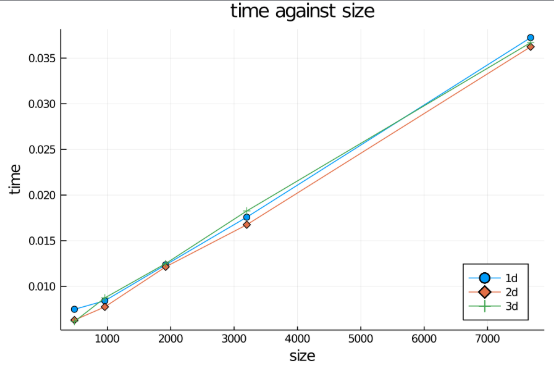
\includegraphics[width=0.6\linewidth]{lineartime.PNG}
\end{figure}
\begin{itemize}
    \item Linear in $n$
    \item Independent of problem dimension
\end{itemize}
\end{frame}

\begin{frame}
\frametitle{What is left}
\begin{itemize}
\item How to choose parameter? (The common method cross validation seems not appropriate.)
\item Getting stuck in Newton's method in barrier method
\item How to verify the solution from the CG-ADMM algorithm?
\end{itemize}
\end{frame}

%------------------------------------------------

\begin{frame}
\frametitle{References}
\footnotesize{
\begin{thebibliography}{99} % Beamer does not support BibTeX so references must be inserted manually as below
\bibitem[Hassanieh, 2012]{p1} Hassanieh, Haitham and Indyk, Piotr and Katabi, Dina and Price, Eric (2012)
\newblock Simple and practical algorithm for sparse Fourier transform
\newblock \emph{Proceedings of the twenty-third annual ACM-SIAM symposium on Discrete Algorithms} 1183--1194.

\bibitem[Tibshirani, 1996]{p2} Tibshirani, Robert (1996)
\newblock Regression shrinkage and selection via the lasso
\newblock \emph{Journal of the Royal Statistical Society: Series B (Methodological)} 58(1) 267--288.

\bibitem[Boyd, 2004]{p3} Boyd, Stephen and Boyd, Stephen P and Vandenberghe, Lieven (2004)
\newblock Convex optimization
\newblock \emph{Cambridge university press}
\end{thebibliography}
}
\end{frame}

%------------------------------------------------

\begin{frame}
\Huge{\centerline{The End}}
\end{frame}

%----------------------------------------------------------------------------------------

\end{document}